\chapter{Les provinces impériales}

Foulez la terre de Tamriel, et voguez à travers le vaste monde !

\section{Archipel de Summerset}

\begin{center}
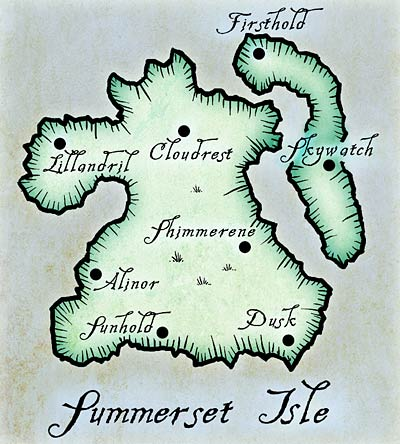
\includegraphics[width=5cm]{images/map_summerset.jpg}
\end{center}

Îles où vivent les Altmers. Beaucoup de paysages semblent vierges, excepté les forêts remaniées par les Altmers pour que les arbres forment de véritables villes, en hauteur, accessibles par des marches, des lianes, ou d'autres moyens (notamment magiques). La tour de Cristal est similaire à celle de la capitale de l'Empire, mais comme son nom l'indique, elle est en cristal, et non en marbre...

\section{Cyrodiil}

\begin{center}
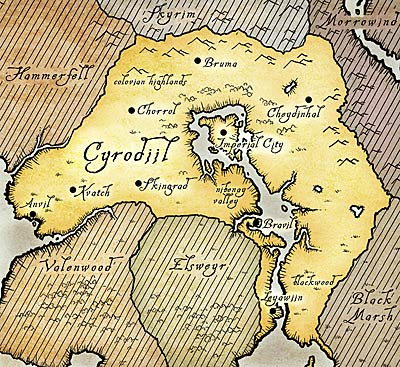
\includegraphics[width=5cm]{images/map_cyrodiil.jpg}
\end{center}

Province centrale, où se sont établis les Impériaux quand ils sont arrivés à Tamriel. Plusieurs sources d'eau provenant des montagnes frontalières se transforment en rivières et forment au milieu de la province un lac, au milieu duquel se trouve la cité impériale. Au sud du lac débute le fleuve qui va jusqu'à la mer. De nombreux petits villages portuaires existent le long de ce fleuve. Les frontières avec les autres provinces sont naturelles, il s'agit soit d'un océan, soit de montagnes… excepté vers les Marais Noirs, mais personne n'y va jamais…

Il y a au moins 7 microclimats différents, des glaciales montagnes du nord aux vignobles près de Skingrad, en passant par les montagnes arides proches de Cheydinhal ...

La capitale de Cyrodiil est également la capitale Impériale.

\section{Elsweyr}

\begin{center}
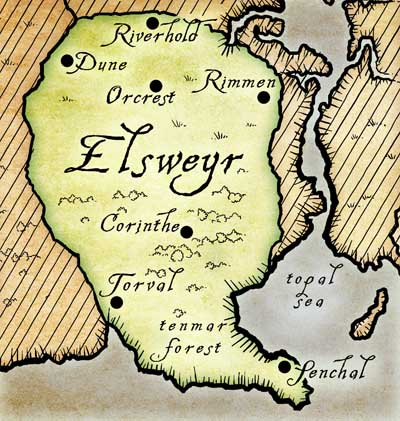
\includegraphics[width=5cm]{images/map_elsweyr.jpg}
\end{center}

Le nord de cette province est fait de marais, alors que le sud est rempli de forêts tropicales. Peu de villes, et si les impériaux n'avaient pas construit quelques villages un peu plus grands, il n'y aurait que des cabanes par-ci par-là.

La capitale est le village de Torval.

\section{Hammerfell}

\begin{center}
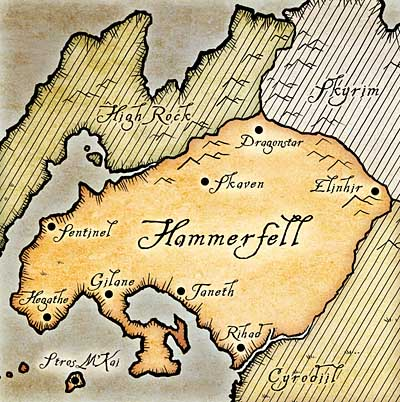
\includegraphics[width=5cm]{images/map_hammerfell.jpg}
\end{center}

Contrée de l'Ouest de Tamriel, bordée par Cyrodiil, Hauteroche et Skyrim. La majorité de ces terres forme le désert d'Alik'r. 

Habitée en premier lieu par le clan Dwemer des Rourken, elle est aujourd'hui l'habitat des rougegardes. À cause du désert et des montagnes, seules les côtes, plus vertes et humides, sont habitées et l'on peut y trouver de grandes cités. Le désert est quant à lui la maison de quelques tribus rougegardes nomades.

Pas de capitale, chaque ville s'auto-gérant, et gérant les relations avec ses voisines.

\section{Highrock}

\begin{center}
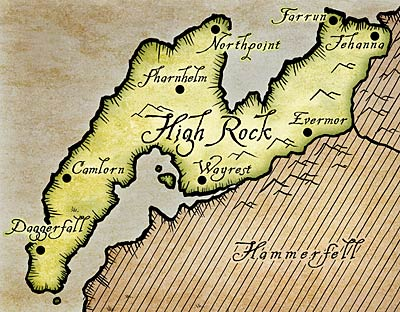
\includegraphics[width=5cm]{images/map_highrock.jpg}
\end{center}

Sur les côtes, cette province est boisée, il y a des prairies, tandis que plus on s'enfonce dans les terres, plus la topologie est irrégulière et les montagnes importantes.

La province est divisée en cités-états, et alors que les bretons occupent quasiment toute la province, les orsimers sont cantonnés dans la cité-état Orsinium. Les lois et valeurs impériales semblent ici faibles, tant les dirigeants des cités-états (y compris ceux d'Orsinium) semblent n'en faire qu'à leur tête.

\section{Blackmarsh}

\begin{center}
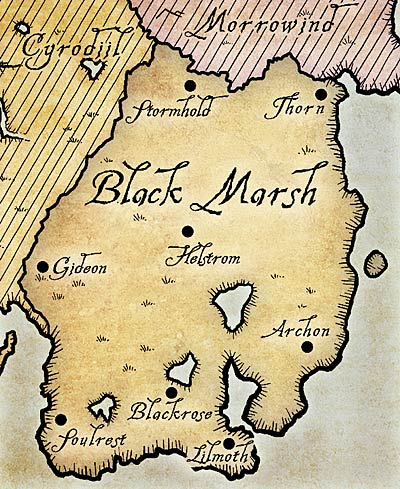
\includegraphics[width=5cm]{images/map_blackmarsh.jpg}
\end{center}

Appelée Argonia par les Mer, cette province n'est que marais toxiques emplis de prédateurs hostiles et redoutables. L'est est un peu plus vert et sec, mais de peu. Et l'Empire, pour avoir écrasé une révolte dans ces marais, sait que jamais plus elle n'enverra de troupes là bas, car si les argoniens sont immunisés contre les toxines des marais, ce n'est pas le cas de toutes les autres races...

Il y a de toutes façons peu de routes, le moyen de transport le plus sûr et le plus rapide est le bateau ...

\section{Morrowind}

\begin{center}
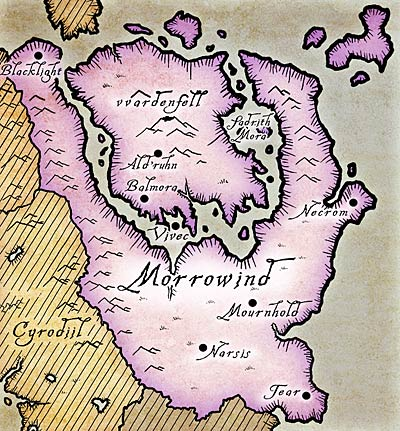
\includegraphics[width=5cm]{images/map_morrowind.jpg}
\end{center}

Des volcans et des conditions de vie horribles pour l'île de Vvarfendell, au centre de la province. Aucun volcan mais des montagnes laides et des conditions de vie tout aussi déplorables pour le reste de la province. Seuls les dunmers et ceux qui veulent se cacher peuvent se plaire dans cette province repoussante, où la majorité des personnes est dunmer. Et quand on n'est pas dunmer, s'aventurer en Morrowind, c'est jouer avec le feu...

Il est connu qu'avant de disparaitre, les Dwemer étaient nombreux dans cette province, car là où se trouve aujourd'hui la montagne rouge se trouvait leur capitale...

Cela s'améliore cependant, car depuis que Dagoth Ur a été tué, l'île commence à se reverdir franchement de ses bordures vers l'intérieur.

La capitale est Almalexia (Connue aussi sous le nom de Longsanglot), située non pas sur Vvarfendell, mais dans les terres.

\section{Skyrim}

\begin{center}
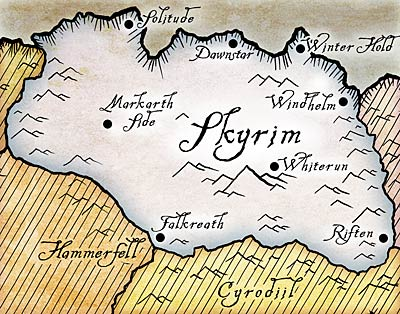
\includegraphics[width=5cm]{images/map_skyrim.jpg}
\end{center}

Cette contrée glaciale, montagneuse et désolée occupe le nord de Tamriel. Bien que son climat soit inhospitalier, comme les steppes, les Nordiques y vivent depuis qu'ils sont arrivés il y a de cela bien longtemps.

Les maisons sont construites en grosses pierres, cerclées et décorées de bois, de manière à conserver le plus de chaleur possible. Dans cette optique l'entrée d'un bâtiment est à la surface, alors que les lieux vitaux (salon, chambre, réception,...) sont dans les sous-sols. Bruma, pourtant en Cyrodiil, a le même genre d'habitation, les gens de Skyrim ayant conseillé les architectes de Cyrodiil.

\section{Valenwood}

\begin{center}
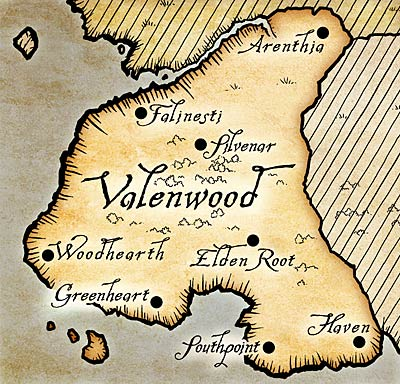
\includegraphics[width=5cm]{images/map_valenwood.jpg}
\end{center}

Valenwood, au sud-ouest de l'Empire, est une contrée emplie de forêts fluviales et de jungles vertes. Elle est bordée au sud et à l'Ouest par la mer, alors que le Nord est bordé par Cyrodiil, et l'Est par Elsweyr. 

Géographiquement, le Guide de Poche de l'Empire décrit ce pays comme "Une mer verte, sans fin, où les cités arboricoles presqu'invisibles fleurissent comme les bourgeons des nombreuses fleurs que l'on peut y trouver". Certaines forêts ont des arbres si grands et forts qu'ils portent sur leurs branches une cité entière, comme c'est le cas de la cité de Falinesti. Il peut être curieux d'expliquer que cette ville migre. En hiver, la forêt se déplace, mue par une magie très ancienne, pour revenir en été à l'endroit où elle se trouvait avant.

